\documentclass{standalone}
\usepackage{tikz}
\usetikzlibrary{patterns, positioning}


\begin{document}
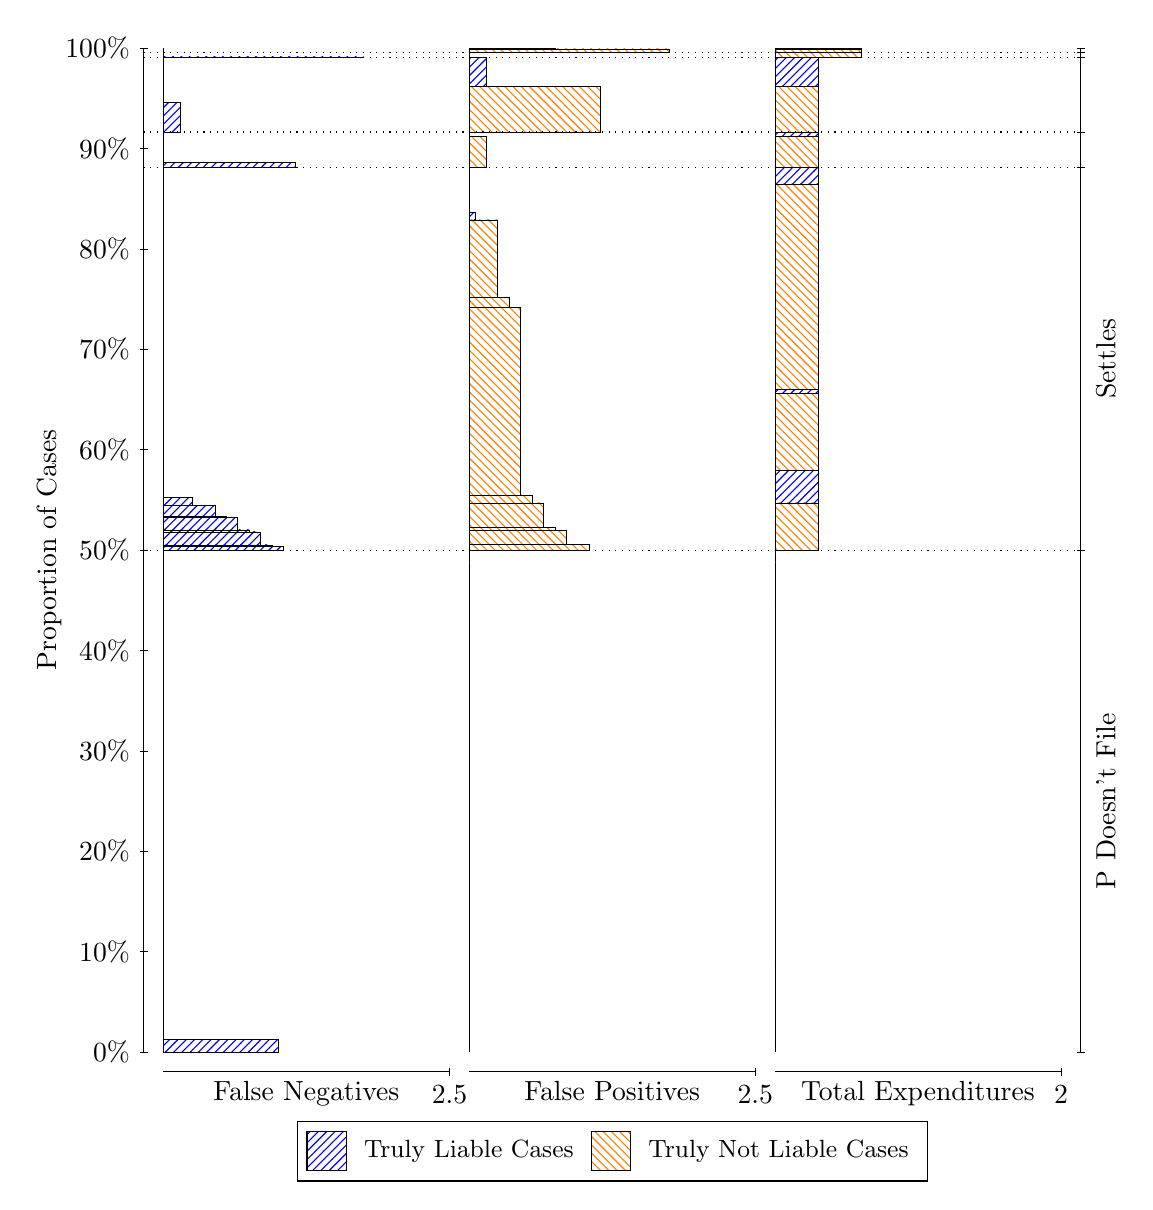
\begin{tikzpicture}
\draw[black, very thin] (1.5,1.75) -- (1.5,14.5);
\node[rotate=90, text=black, anchor=center] at (0.3, 8.125) {Proportion of Cases};
\draw[black, very thin] (1.45,1.75) -- (1.55,1.75);
\node[text=black, anchor=east] at (1.45, 1.75) {0\%};
\draw[black, very thin] (1.45,3.025) -- (1.55,3.025);
\node[text=black, anchor=east] at (1.45, 3.025) {10\%};
\draw[black, very thin] (1.45,4.3) -- (1.55,4.3);
\node[text=black, anchor=east] at (1.45, 4.3) {20\%};
\draw[black, very thin] (1.45,5.575) -- (1.55,5.575);
\node[text=black, anchor=east] at (1.45, 5.575) {30\%};
\draw[black, very thin] (1.45,6.85) -- (1.55,6.85);
\node[text=black, anchor=east] at (1.45, 6.85) {40\%};
\draw[black, very thin] (1.45,8.125) -- (1.55,8.125);
\node[text=black, anchor=east] at (1.45, 8.125) {50\%};
\draw[black, very thin] (1.45,9.4) -- (1.55,9.4);
\node[text=black, anchor=east] at (1.45, 9.4) {60\%};
\draw[black, very thin] (1.45,10.675) -- (1.55,10.675);
\node[text=black, anchor=east] at (1.45, 10.675) {70\%};
\draw[black, very thin] (1.45,11.95) -- (1.55,11.95);
\node[text=black, anchor=east] at (1.45, 11.95) {80\%};
\draw[black, very thin] (1.45,13.225) -- (1.55,13.225);
\node[text=black, anchor=east] at (1.45, 13.225) {90\%};
\draw[black, very thin] (1.45,14.5) -- (1.55,14.5);
\node[text=black, anchor=east] at (1.45, 14.5) {100\%};

\draw[black, very thin] (13.4,1.75) -- (13.4,14.5);
\draw[black, very thin] (13.35,1.75) -- (13.45,1.75);
\node[anchor=west] at (13.35, 1.75) {};
\draw[black, very thin] (13.35,8.122) -- (13.45,8.122);
\node[anchor=west] at (13.35, 8.122) {};
\draw[black, very thin] (13.35,12.988) -- (13.45,12.988);
\node[anchor=west] at (13.35, 12.988) {};
\draw[black, very thin] (13.35,13.433) -- (13.45,13.433);
\node[anchor=west] at (13.35, 13.433) {};
\draw[black, very thin] (13.35,14.384) -- (13.45,14.384);
\node[anchor=west] at (13.35, 14.384) {};
\draw[black, very thin] (13.35,14.448) -- (13.45,14.448);
\node[anchor=west] at (13.35, 14.448) {};
\draw[black, very thin] (13.35,14.5) -- (13.45,14.5);
\node[anchor=west] at (13.35, 14.5) {};

\draw[black, very thin, pattern color=blue, pattern=north east lines] (1.75,1.75) rectangle (3.2033,1.9075);
\draw[black, very thin, pattern color=orange, pattern=north west lines] (1.75,1.9075) rectangle (1.75,8.122);
\draw[black, very thin, pattern color=blue, pattern=north east lines] (1.75,8.122) rectangle (3.276,8.1669);
\draw[black, very thin, pattern color=blue, pattern=north east lines] (1.75,8.1669) rectangle (3.1307,8.1902);
\draw[black, very thin, pattern color=blue, pattern=north east lines] (1.75,8.1902) rectangle (2.9853,8.3538);
\draw[black, very thin, pattern color=blue, pattern=north east lines] (1.75,8.3538) rectangle (2.84,8.3804);
\draw[black, very thin, pattern color=blue, pattern=north east lines] (1.75,8.3804) rectangle (2.6947,8.5372);
\draw[black, very thin, pattern color=blue, pattern=north east lines] (1.75,8.5372) rectangle (2.5493,8.5536);
\draw[black, very thin, pattern color=blue, pattern=north east lines] (1.75,8.5536) rectangle (2.404,8.6947);
\draw[black, very thin, pattern color=blue, pattern=north east lines] (1.75,8.6947) rectangle (2.1133,8.7944);
\draw[black, very thin, pattern color=orange, pattern=north west lines] (1.75,8.7944) rectangle (1.75,12.988);
\draw[black, very thin, pattern color=blue, pattern=north east lines] (1.75,12.988) rectangle (3.4213,13.043);
\draw[black, very thin, pattern color=orange, pattern=north west lines] (1.75,13.043) rectangle (1.75,13.433);
\draw[black, very thin, pattern color=blue, pattern=north east lines] (1.75,13.433) rectangle (1.968,13.808);
\draw[black, very thin, pattern color=orange, pattern=north west lines] (1.75,13.808) rectangle (1.75,14.384);
\draw[black, very thin, pattern color=blue, pattern=north east lines] (1.75,14.384) rectangle (4.2933,14.388);
\draw[black, very thin, pattern color=orange, pattern=north west lines] (1.75,14.388) rectangle (1.75,14.448);
\draw[black, very thin, pattern color=orange, pattern=north west lines] (1.75,14.448) rectangle (1.75,14.488);
\draw[black, very thin, pattern color=blue, pattern=north east lines] (1.75,14.488) rectangle (1.75,14.5);
\draw[black, very thin, pattern color=orange, pattern=north west lines] (5.6333,1.75) rectangle (5.6333,7.9645);
\draw[black, very thin, pattern color=blue, pattern=north east lines] (5.6333,7.9645) rectangle (5.6333,8.122);
\draw[black, very thin, pattern color=orange, pattern=north west lines] (5.6333,8.122) rectangle (7.1593,8.1983);
\draw[black, very thin, pattern color=orange, pattern=north west lines] (5.6333,8.1983) rectangle (6.8687,8.3741);
\draw[black, very thin, pattern color=orange, pattern=north west lines] (5.6333,8.3741) rectangle (6.7233,8.4116);
\draw[black, very thin, pattern color=orange, pattern=north west lines] (5.6333,8.4116) rectangle (6.578,8.723);
\draw[black, very thin, pattern color=orange, pattern=north west lines] (5.6333,8.723) rectangle (6.4327,8.8217);
\draw[black, very thin, pattern color=orange, pattern=north west lines] (5.6333,8.8217) rectangle (6.2873,11.209);
\draw[black, very thin, pattern color=orange, pattern=north west lines] (5.6333,11.209) rectangle (6.142,11.335);
\draw[black, very thin, pattern color=orange, pattern=north west lines] (5.6333,11.335) rectangle (5.9967,12.316);
\draw[black, very thin, pattern color=blue, pattern=north east lines] (5.6333,12.316) rectangle (5.706,12.416);
\draw[black, very thin, pattern color=blue, pattern=north east lines] (5.6333,12.416) rectangle (5.6333,12.988);
\draw[black, very thin, pattern color=orange, pattern=north west lines] (5.6333,12.988) rectangle (5.8513,13.379);
\draw[black, very thin, pattern color=blue, pattern=north east lines] (5.6333,13.379) rectangle (5.6333,13.433);
\draw[black, very thin, pattern color=orange, pattern=north west lines] (5.6333,13.433) rectangle (7.3047,14.009);
\draw[black, very thin, pattern color=blue, pattern=north east lines] (5.6333,14.009) rectangle (5.8513,14.384);
\draw[black, very thin, pattern color=orange, pattern=north west lines] (5.6333,14.384) rectangle (5.6333,14.444);
\draw[black, very thin, pattern color=blue, pattern=north east lines] (5.6333,14.444) rectangle (5.6333,14.448);
\draw[black, very thin, pattern color=orange, pattern=north west lines] (5.6333,14.448) rectangle (8.1767,14.488);
\draw[black, very thin, pattern color=blue, pattern=north east lines] (5.6333,14.488) rectangle (6.7233,14.5);
\draw[black, very thin, pattern color=orange, pattern=north west lines] (9.5167,1.75) rectangle (9.5167,7.9645);
\draw[black, very thin, pattern color=blue, pattern=north east lines] (9.5167,7.9645) rectangle (9.5167,8.122);
\draw[black, very thin, pattern color=orange, pattern=north west lines] (9.5167,8.122) rectangle (10.062,8.723);
\draw[black, very thin, pattern color=blue, pattern=north east lines] (9.5167,8.723) rectangle (10.062,9.137);
\draw[black, very thin, pattern color=orange, pattern=north west lines] (9.5167,9.137) rectangle (10.062,10.118);
\draw[black, very thin, pattern color=blue, pattern=north east lines] (9.5167,10.118) rectangle (10.062,10.163);
\draw[black, very thin, pattern color=orange, pattern=north west lines] (9.5167,10.163) rectangle (10.062,12.775);
\draw[black, very thin, pattern color=blue, pattern=north east lines] (9.5167,12.775) rectangle (10.062,12.988);
\draw[black, very thin, pattern color=orange, pattern=north west lines] (9.5167,12.988) rectangle (10.062,13.379);
\draw[black, very thin, pattern color=blue, pattern=north east lines] (9.5167,13.379) rectangle (10.062,13.433);
\draw[black, very thin, pattern color=orange, pattern=north west lines] (9.5167,13.433) rectangle (10.062,14.009);
\draw[black, very thin, pattern color=blue, pattern=north east lines] (9.5167,14.009) rectangle (10.062,14.384);
\draw[black, very thin, pattern color=orange, pattern=north west lines] (9.5167,14.384) rectangle (10.607,14.444);
\draw[black, very thin, pattern color=blue, pattern=north east lines] (9.5167,14.444) rectangle (10.607,14.448);
\draw[black, very thin, pattern color=orange, pattern=north west lines] (9.5167,14.448) rectangle (10.607,14.488);
\draw[black, very thin, pattern color=blue, pattern=north east lines] (9.5167,14.488) rectangle (10.607,14.5);
\draw[black, dotted] (1.5,8.122) -- (13.4,8.122);
\draw[black, dotted] (1.5,12.988) -- (13.4,12.988);
\draw[black, dotted] (1.5,13.433) -- (13.4,13.433);
\draw[black, dotted] (1.5,14.384) -- (13.4,14.384);
\draw[black, dotted] (1.5,14.448) -- (13.4,14.448);
\draw[black, very thin] (1.75,1.5) -- (5.3833,1.5);
\node[text=black, anchor=north] at (3.5667, 1.5) {False Negatives};
\draw[black, very thin] (5.3833,1.45) -- (5.3833,1.55);
\node[text=black, anchor=north] at (5.3833, 1.45) {2.5};

\draw[black, very thin] (5.6333,1.5) -- (9.2667,1.5);
\node[text=black, anchor=north] at (7.45, 1.5) {False Positives};
\draw[black, very thin] (9.2667,1.45) -- (9.2667,1.55);
\node[text=black, anchor=north] at (9.2667, 1.45) {2.5};

\draw[black, very thin] (9.5167,1.5) -- (13.15,1.5);
\node[text=black, anchor=north] at (11.333, 1.5) {Total Expenditures};
\draw[black, very thin] (13.15,1.45) -- (13.15,1.55);
\node[text=black, anchor=north] at (13.15, 1.45) {2};

\node[text=black, centered, rotate=90] at (13.72, 4.936) {P Doesn't File};
\node[text=black, centered, rotate=90] at (13.72, 10.555) {Settles};





\draw (7.449999999999999,1.5) node[draw=none] (baseCoordinate) {};
\begin{scope}[align=center]
        \matrix[scale=0.5, draw=black, below=0.5cm of baseCoordinate, nodes={draw}, column sep=0.1cm]{
            \node[rectangle, draw, minimum width=0.5cm, minimum height=0.5cm, pattern color=blue, pattern=north east lines] {}; &
            \node[draw=none, font=\small, text=black] (B) {Truly Liable Cases}; &
            \node[rectangle, draw, minimum width=0.5cm, minimum height=0.5cm, pattern color=orange, pattern=north west lines] {}; &
            \node[draw=none, font=\small, text=black] (B) {Truly Not Liable Cases}; \\
            };
\end{scope}

\end{tikzpicture}
\end{document}